\documentclass[a4paper]{article}
\usepackage[utf8]{inputenc}
\usepackage{wrapfig}
\usepackage{caption}
\usepackage{graphicx}
\usepackage{geometry}
 \geometry{
 a4paper,
 total={210mm,297mm},
 left=20mm,
 right=20mm,
 top=20mm,
 bottom=20mm,
 }

\pdfinfo{
  /Title    (Building Serious Games - Design4Health)
  /Author   (Ralf Nieuwenhuizen, David Prihoda, Ismini Psychoula, Arnold Schutter, Shen Shuheng)
  /Creator  (Ralf Nieuwenhuizen, David Prihoda, Ismini Psychoula, Arnold Schutter, Shen Shuheng)
  /Producer (Ralf Nieuwenhuizen, David Prihoda, Ismini Psychoula, Arnold Schutter, Shen Shuheng)
  /Subject  (Building Serious Games)
}


%Game design report (no more than 8-10 pages)
%1. serious game (purpose and reality)
%- purpose of the game; what does it need to bring about beyond the context of the game?
%- what is the strategy you chose to achieve that purpose?; how does it work, and why?
%- what is the role of the main operations and game elements in that strategy? how are these elements
%kept in balance?
%- describe the model you have developed for your simulation, and explain the choices made
%2. serious game (play)
%- description of the game concept; goal(s) in the game
%- main elements in the game mechanics; game rules
%- essential feedback elements (in relation to the game goals)
%- challenges and dilemmas presented to the player
%- types of choices and actions available (and their role in relation to the game purpose)
%3. from prototype to the final game (up scaling)
%- what was left out in the prototype? what's the roadmap to the final game? what are the main
%challenges on that path?
%- (non-technical) recommendations and warnings

\title{Building Serious Games: Final Game Design}
\author{
	R. Nieuwenhuizen \and
    D. Prihoda  \and
	I. Psychoula \and
	A.S.C. Schutter \and
	S. Shen
 }
\date{January 2015}

\begin{document}

\maketitle

\begin{abstract}
In this article our project group describes the final version of the game PhysioFun. The game encourages the users to live a healthier life. We aim to reach this goal by stimulating the user to execute exercises, provide feedback and give further suggestions for a healthy lifestyle. \\
The progress of the user is integrated in the storyline of the game, which should eccentrically motivate the user to keep up the good behavior. The intrinsic motivation to live healthy is supported by supplying information and personal feedback. All the exercises serve different goals and train different bodyparts, this information is provided to the user.  \\
The engaging interaction of the user with the game is supported by the sensors of the smartphone. The sensors are used to provide feedback to the user and give the feeling that all the effort is worth it.
\end{abstract}

\section{Introduction}
Nowadays, people are getting more and more stuck behind their desks or on the couch, which is the cause for many diseases. Physiofun is a mobile phone game designed to encourage the users to exercise regularly. The user will try to develop a farm in space, by completing real life exercises.\\
\\
The idea for the application originated from the project specifications set to us by Design4Health, a company that aims to ``apply user-centered design tools and methods to the field of healthcare. Through a careful study of digital touch-points, behavioral science and a combination of digital and physical products to shape a new and better healthcare experience.''\\
\\
The report will start off explaining the various design decisions we have made, and why we have made them. After that, the technologies used will be explained, followed by the game structure along with all the components in the game. Next there will be a part about the user interface, followed by a section about the sensors used to measure the exercises. The report will conclude with challenges we had during the development, and technical recommendations towards a real serious game, which is ready for the market, you can regard this as a ``wishlist''.

\section{Purpose of the game}
\label{chap:GamePurpose}
%1. serious game (purpose and reality)
%- purpose of the game; what does it need to bring about beyond the context of the game?
%- what is the strategy you chose to achieve that purpose?; how does it work, and why?
%- what is the role of the main operations and game elements in that strategy? how are these elements kept in balance?
%- describe the model you have developed for your simulation, and explain the choices made

The game is designed to be fun and engaging for users, a necessary characteristic to reach the actual purpose of the game: \textit{Stimulating a healthy lifestyle}. 

\subsection{Real life implications}
From a real life point of view, the user is encouraged by the game to perform isolated exercises that are carefully selected to cover all body regions. The user is also able to set personal goals by choosing to perform sets of exercises focused on a specific body region. All the real life implications of performing exercises are explicitly mentioned in the game, while being seamlessly incorporated in the storyline. Finally, the game does stimulate the user to think about the current lifestyle.

\subsection{Way of implementation}
Different game elements help to include the real life implications in the game and communicate them to the user. To be able to provide specific feedback, the body is categorized in $5$ specific body parts: The back, the chest, the abs, the arms and the legs. \\
\\
The exercises are specifically selected to train the different body parts to support the user's general fitness. The challenges include specific sets of exercises and can voluntarily be selected by the user. The user is able to focus on specific body parts by selecting challenges which contain exercises for that body part. The progression of the user is represented in the B.O.D.Y. which is showing the progress for each specific body part and can be compared to the historical progress via a statistics screen. \\
\\
To support a healthy lifestyle outside the game, the user is motivated to think about it by daily task provided by the mentor. This daily task is introduced to trigger the user to think about a healthy lifestyle while not playing the game. 

\subsubsection{Exercises}
The game contains a variety of exercises with different aims. The exercises contain information about the way they should be executed and which groups of muscles are trained. During the execution of the exercise, a smartphone is used to measure the movements and to provide acoustic feedback. The exercises are chosen in cooperation with a physiotherapist, who provided feedback on how to execute them correctly.

\subsubsection{Challenges}
Challenges combine exercises into a workout in a playful way. This is an easy way for the user to keep his whole body strong and fit, and prevent injuries. Challenges also give users the opportunity to do exercises at each time of the day, without having to wait for crops or livestock to get ready for harvest. A challenge without requirements is available as well, which lets the user walk a certain amount of steps. This is a good way to earn extra money when all is spent. This is a metaphor of \emph{``no matter how physically impaired you are, you can always take some steps to get better"}. 

\subsubsection{B.O.D.Y.}
The Bionic Outer Dimension Yeosuit (B.O.D.Y.) represents the progress of the real life body of the user. By executing the exercises the user earns experience points for the represented body parts. When sufficient experience points are earned for each body part, the B.O.D.Y.-level will increase, allowing the user to do more challenges and clone more crops and livestock. This is similar to the way a better general fitness allows someone to do more demanding tasks in real life. Every time you open the B.O.D.Y. screen you will be advised to give attention to your weakest body part.

\subsubsection{Statistics}
While the user progresses in the game, it motivates to have a look back in history on all efforts that have been made. Therefore the game reflects the user's long-term progress, encouraging to continue exercising regularly throughout the day and also to focus on all different body regions equally. 

\subsubsection{Daily tasks}
Every day, the user is challenged to do a real life task, such as taking the stairs instead of the elevator. These tasks are not obtrusive nor enforced, but are there to make the user aware of living healthy outside of the game, providing easy tasks to make everyday life more healthy. 

\section{Gameplay}
%2. serious game (play)
%- description of the game concept; goal(s) in the game
%- main elements in the game mechanics; game rules
%- essential feedback elements (in relation to the game goals)
%- challenges and dilemmas presented to the player
%- types of choices and actions available (and their role in relation to the game purpose)

In this chapter the game is explained in more detail. The game is designed to be engaging to support the real purpose as explained in chapter~\ref{chap:GamePurpose}. This chapter starts with the game story and an explanation of the game play. Subsequently the features of the game are explained. 

\subsection{Game Story}
The game starts with a story to get the user into the game. 
\\
\begin{wrapfigure}{l}{150px}
  \vspace{-30pt}
	\begin{center}
		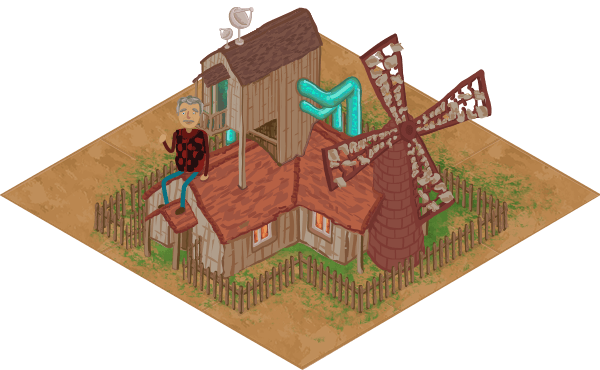
\includegraphics[width=150px]{images/farm.png}
	\end{center}
  \vspace{-10pt}
	\caption{The farm}
  \vspace{-20pt}
	\label{fig:farm}
\end{wrapfigure}
\textit{2542 AD. Your uncle was one of the first people to buy land in an unknown planet and decided to turn it into a farm to facilitate the earth's growing needs of food. Your uncle made the farm very profitable and he produced the best products available on earth. You received a mail telling you that your uncle had left you the farm already years ago. The fields on planet Yeo are unused and empty. Are you able to make the farm successful again?}
\\\\
\subsection{Gameplay}
The user is a novice farmer in the game and is instructed by a virtual physiotherapist, an old farmer called Phil. Phil instructs the user to learn and perform different types of exercises regularly that help to stay healthy in real life. Executing the exercises is also necessary to progress in the game. By cloning crops and livestock the user can become a more skilled farmer and revive the company. 
\\\\
The game mechanics are shown in Figure~\ref{fig:gameconcept}. The central point is the exercise, which influences all the progress in the game.

\begin{figure}[h]
	\centering
		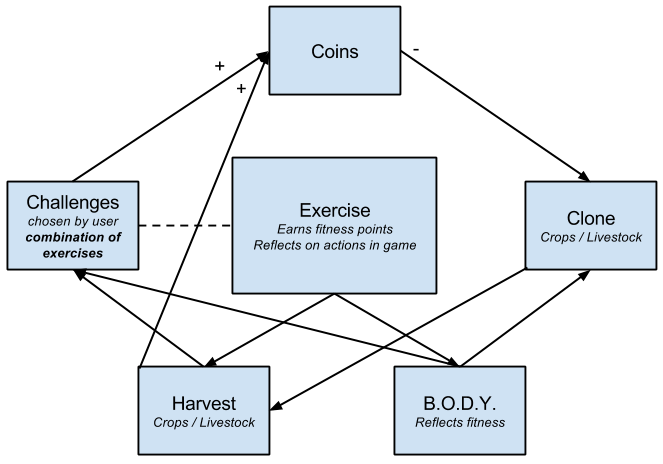
\includegraphics[width=0.80\textwidth]{images/gameconcept.png}
	\caption{Game mechanics}
	\label{fig:gameconcept}
\end{figure}

To clone crops or livestock on the farm, the farmer needs sufficient coins to buy them. Coins can be earned by harvesting products or by completing challenges. The user can pay coins to clone the crops or livestock and place them on tiles in the map. In a certain time interval the crops are ripe and can be harvested and livestock products can be gathered. In order to do this, specific exercises are to be executed in real life. 
\\\\
Challenges are separate stories and require the execution of a set of exercises focused on a specific body region or on the full body. Most of the challenges require you to harvest some items before starting them.
\\\\
The farmer is equipped with a Bionic Outer Dimension Yeosuit (B.O.D.Y.) as described in chapter \ref{chap:GamePurpose}. The B.O.D.Y. reflects all the exercises the user has executed. For example, after performing an exercise that focuses on chest muscles, experience points are added to the B.O.D.Y. for the chest. Once the user has enough experience points for each body part, the level of the B.O.D.Y. is increased. This way, the user is informed about which body regions have to be improved and need more focus in the future. An upgrade of the level of the B.O.D.Y. allows the user to clone more products and unlocks new challenges.
\\\\
More details about each of these components will be given in paragraph~\ref{subsec:GameFeatures}.

\subsection{Example game scenario}
This section provides an example of the game play. In this example, the user clones a space apple tree with his money and plants it on any available tile on the map. After a few hours the apples can be harvested, additionally the user can request for a notification to be informed. To harvest the apples, the user has to execute an exercise for picking apples. The mentor gives a description of the exercise in detail and also show how to execute the exercise properly for the users less interested in reading the description. Once the apples are harvested, the user receives the corresponding reward in coins and the harvested space apples are added to the inventory. These space apples might be used to start new challenges or feed the Piggiums, the cloned pigs that are exported to space.

%--List of features explained--
\subsection{Game features}
\label{subsec:GameFeatures}
The sections below describe all game features and their specifications more extensively. This may differ from the original game design document, as several features were left out of the game for varying reasons. These will be discussed in paragraph~\ref{sec:FutureWork}.

\subsubsection{The overview}
At the start of the game, the user sees an introductional story before the farm is shown. A short explanation of the game is given and the B.O.D.Y. is introduced to make the purpose of the game clear. After these introductions the player is ready to start his adventure.
\\\\
Now the farm will be introduced to the user and the uncle is awaiting him there. The amount of space around the farm is fixed throughout the duration of the game. The user is asked by Phil to clone a crop, harvest the crop and finish a challenge. After doing these tasks the user has explored the most important features of the game and should be able to continue without further help. From now on, Mentor Phil provides the user with a daily task to help aiming for a healthy lifestyle. 
\\\\
A screenshot of what the map looks like is shown in Figure~\ref{fig:map}.

\begin{figure}[h]
	\centering
		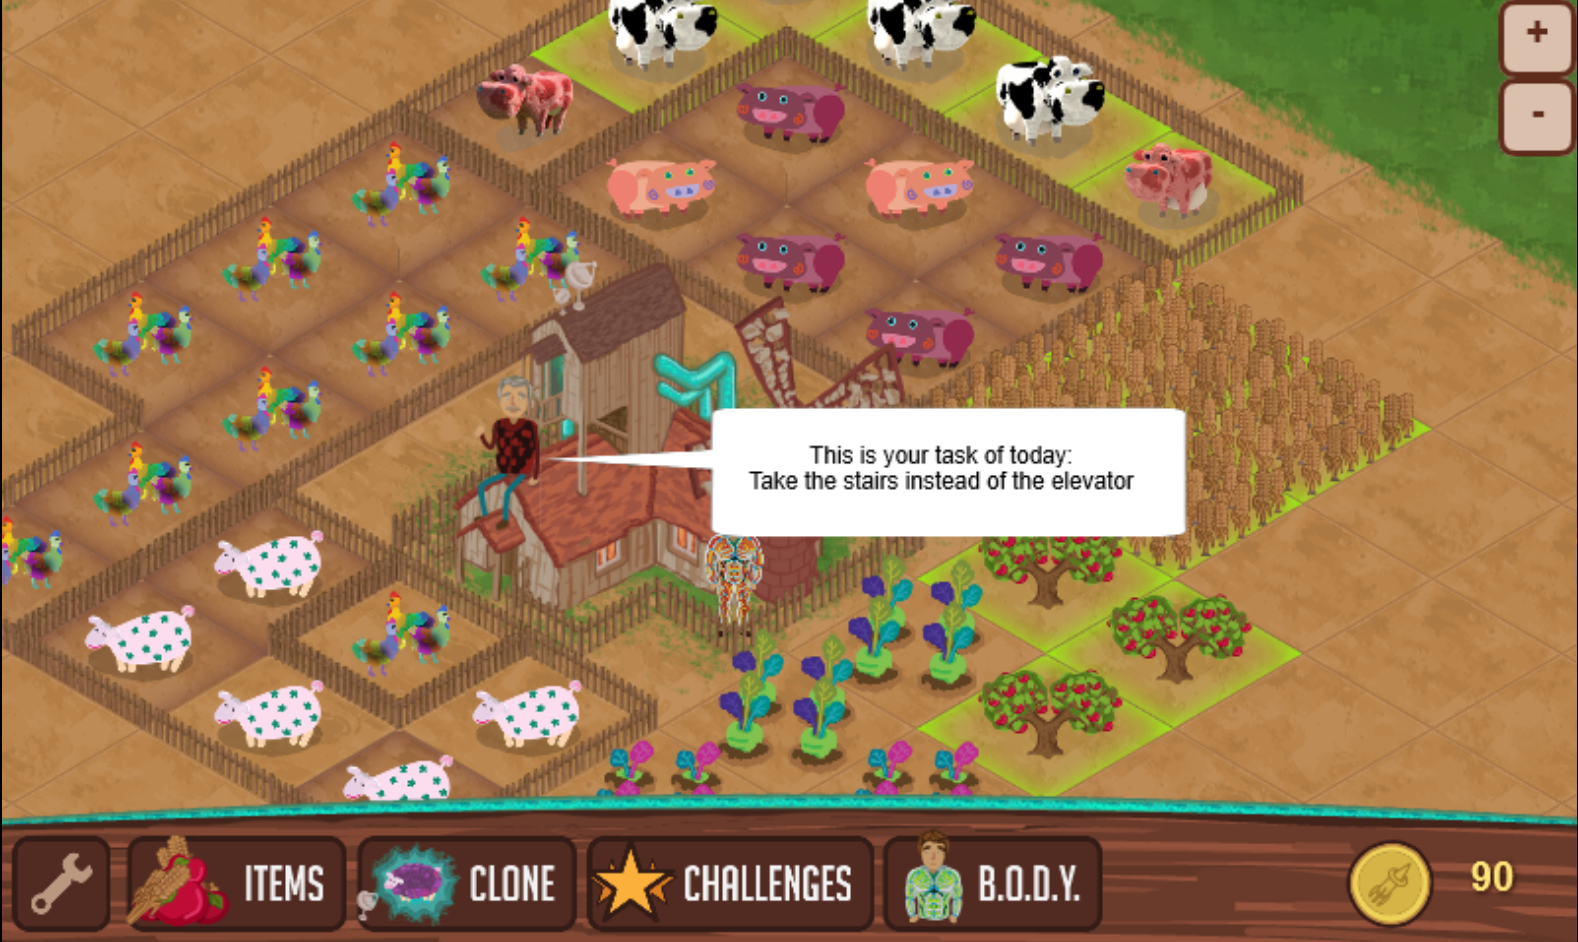
\includegraphics[width=0.80\textwidth]{images/map.png}
	\caption{The map overview}
	\label{fig:map}
\end{figure}

\subsubsection{Mentor Phil}
Once you get to the farm, you discover there is a very old friend of your uncle's, Phil, who is around 60 years old, but still very much in shape. He will serve as your mentor and "personal coach" in the game. Phil explains the purpose and shows the correct execution of each exercise to you. During the game, the mentor and the player will become friends and ``partners in exercise''.

\subsubsection{The farmer}
In the game, the player is impersonated by a farmer. The farmer wears the B.O.D.Y. which is upgraded according to the performed exercises.

\subsubsection{Bionic Outer Dimension Yeosuit}
Apart from the advice part that the player gets from Phil, he also gets reflection of his progress in the game in the form of a ``B.O.D.Y.''. The player has a list of points, one for each body part (arms, legs, abs, back, chest), and each finished exercise will yield some points for a specific body part. When the points for each body part have reached a certain amount, the player is awarded an upgrade of the level of his B.O.D.Y. The upgrade depends on the body part with the least experience points (a chain is as strong as its weakest link). This way, the player will notice when he's focusing too much on one or several body parts and will be motivated to also focus on the other parts. Now the player has a choice in the exercises he performs, but is motivated to make a balanced scheme. 
\\\\
The level of the player is defined by the progress of the B.O.D.Y. In this way, the B.O.D.Y. gives an indication of the progress in the game and the physical performance.  A higher level gives the player more skills and unlocks new crops and livestock.
\\\\
A screenshot of what the B.O.D.Y. looks like is shown in Figure~\ref{fig:body}. As you can see in this image, the player is somewhat behind on his back exercises.

\begin{figure}[h]
	\centering
		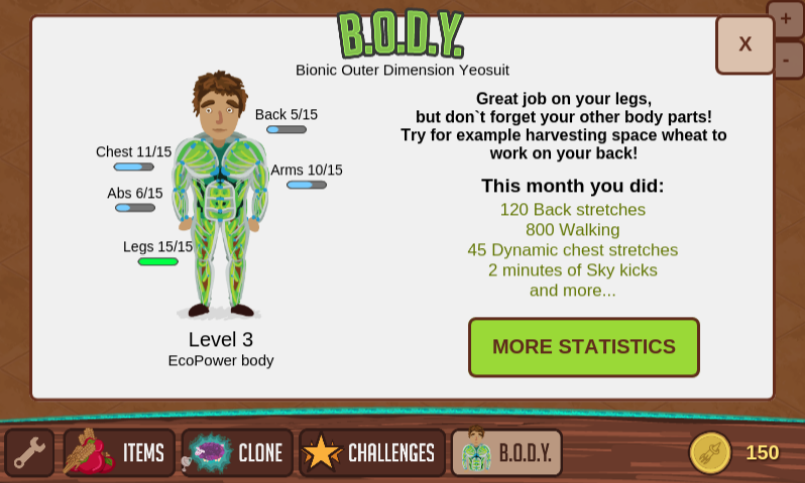
\includegraphics[width=0.80\textwidth]{images/SceneBody.png}
	\caption{The B.O.D.Y.}
	\label{fig:body}
\end{figure}

\subsubsection{Exercises}
During the game, players are asked to execute several exercises in real life. These exercises are necessary for them to harvest a crop, or to exploit the livestock. Prior to each exercise a clear explanation is shown about the movement the player has to perform demonstrated by a drawing of the mentor. The phone is used to measure the execution of the exercise and is handheld by the player. The accelerometer of the phone measures the movement. There are also exercises in the challenges, which are described in the next section. Most of those exercises are measured by a stopwatch, trusting the player's own motivation to execute them correctly. After completing an exercise, the player will be informed which body parts he has exercised by an overview of how much the B.O.D.Y. has improved.
\\\\
A screenshot of what an active exercise looks like is shown in Figure~\ref{fig:exercise}.

\begin{figure}[h]
	\centering
		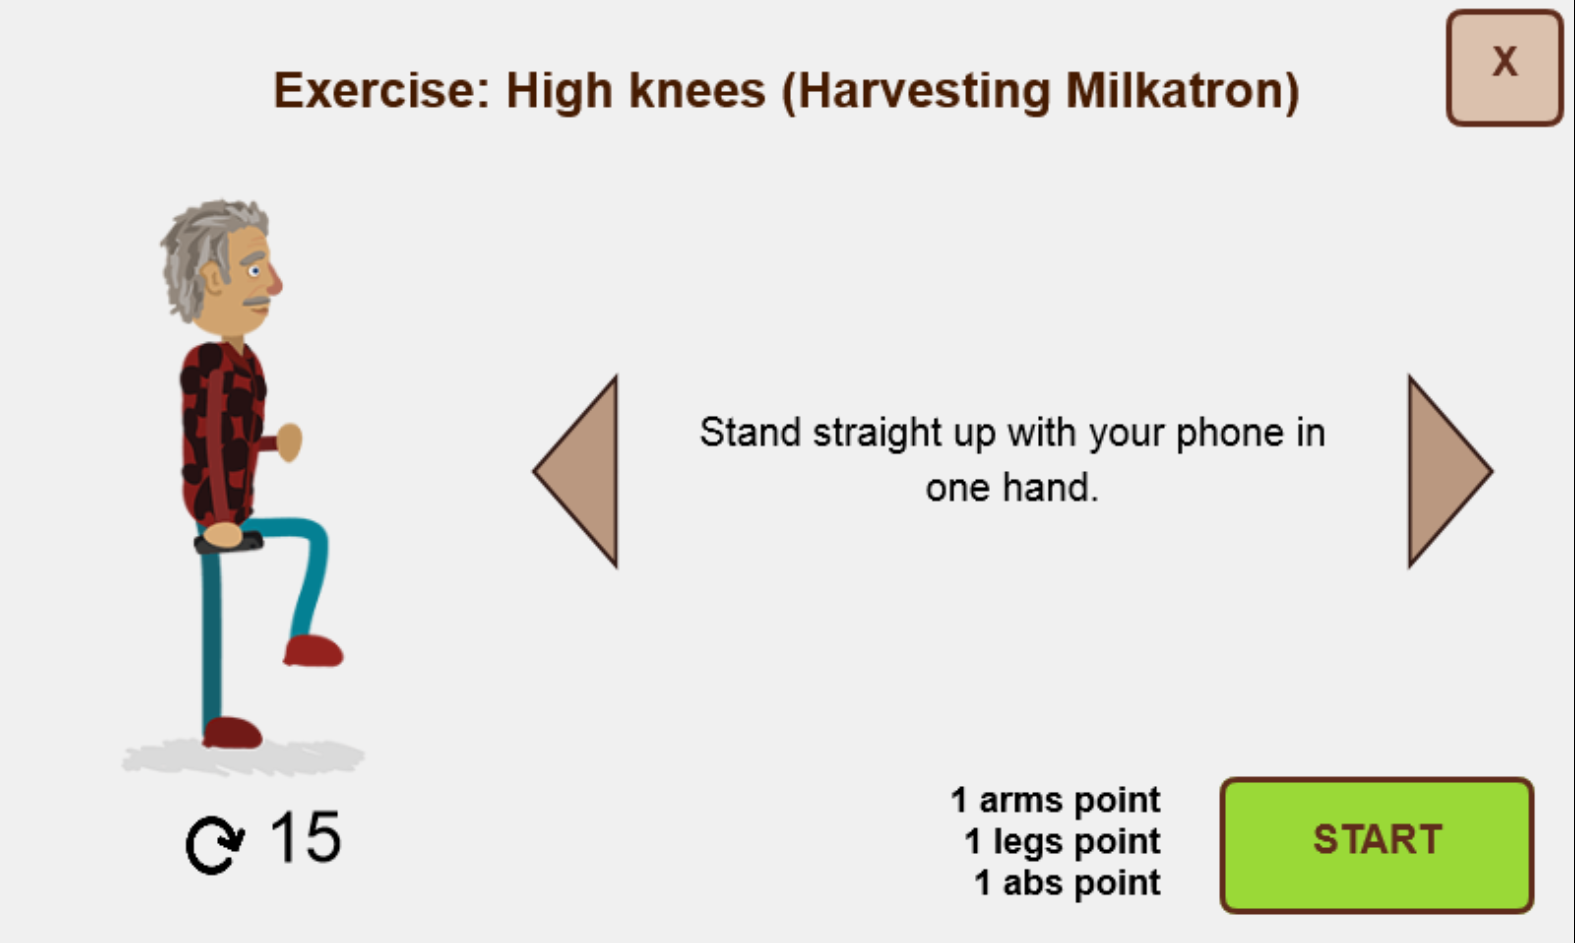
\includegraphics[width=0.80\textwidth]{images/exercise.png}
	\caption{Doing an exercise}
	\label{fig:exercise}
\end{figure}

\paragraph{List of exercises}
A list of current implemented exercises is shown below, categorized by exercises which are measured with the accelerometer and which are timed.
\begin{itemize}
\item Accelerometer exercises %List of accelerometer exercises
\begin{enumerate}
\item Walking
\item Arm stretches
\item Back stretches
\item Sit-ups
\item Dynamic chest stretches
\item Rocket jumps
\item High knees
\item Bear hug crunches
\item Mason twists
\item Wall flying
\item Wall ear touches
\item Wall arm pulling
\end{enumerate}
\item Timed exercises %List of timed exercises
\begin{enumerate}
\item Push ups on knees
\item Push ups
\item Sky kicks
\item Squats
\end{enumerate}
\end{itemize}

\subsubsection{Challenges}
The player has a list of challenges from which he can pick one at anytime and execute that to receive bonus coins. These challenges have an underlying set of exercises that can either be focused on one body part, or they can be a complete body workout. The mentor will explain about that. Challenges are proposed to the player as an appealing task in the game, for example to make a spaceapple pie for your neighbouring Yeowoman that is ill. The player would have to perform some exercises that would be needed to get the ingredients for the space pie, and by doing that he would have completed a workout without noticing. The mentor will inform the player of that afterwards, to raise awareness.
\\\\
You can pick a challenge from the list of available challenges, and you can start it only when you have the required items. These items are used when you do the challenge, so you will not be able to get them back once you have started. After starting the challenge the items are subtracted from your inventory and you can do the required exercises, one at a time. This can be paused anytime, but you will not be able to do any other challenges in the meantime.
\\\\
A screenshot of what an active challenge looks like is shown in Figure~\ref{fig:challenge}.

\begin{figure}[h]
	\centering
		
\includegraphics[width=0.80\textwidth]{images/challenge.png}
	\caption{Doing a challenge}
	\label{fig:challenge}
\end{figure}

\paragraph{Example challenges}
In the current version $8$ challenges are available:
\begin{itemize}
\item Space forest walk
\item Space apple pie
\item Space cookie
\item Woolysocks
\item Carrot pie
\item Apple Sweater
\item Carrot Rocket
\item Strawberry milkshake
\end{itemize}

\subsubsection{Money}
When the game begins the player is provided 150 coins to start developing his farm. After that first allowance he can earn more money by harvesting or by completing challenges. There is also a daily bonus, to reward the players for getting back every day. There might be an occasion, when your crops have died and you have no money nor items left. In that occasion there is a free challenge, which lets you walk around for a while, and which gives you enough money to make a small start again.

\subsubsection{Cloning}
Each type of crop has a name, a cost, a revenue that it yields when harvested and the time it takes for it to grow. Plants will only last one harvest and have to be harvested soon enough (e.g. 12-36 hours, depending on their level), or they will rot away. Trees last multiple harvests.
\\\\
Each type of livestock has a name, a cost, a revenue it yields when exploited and the time it takes for it to be ready (for example milking a Milkatron every 6 hours will produce a bottle of milk and 100 coins). In contrast to the crops, livestock will always stay, it will not die when you don't feed it. To get revenue from livestock, you have to feed them and after a while you will be able to exploit them.
\\\\
All sorts of crops and livestock have a specific exercise attached to them, which the user has to perform to harvest it. The name of the exercise, a preview of the execution, and the amount of experience points it yields are shown on the details screen of the crop or livestock.
\\\\
A screenshot of what the cloning view looks like is shown in Figure~\ref{fig:cloning} and a list of available crops and livestock is shown below.

\begin{figure}[h]
	\centering
		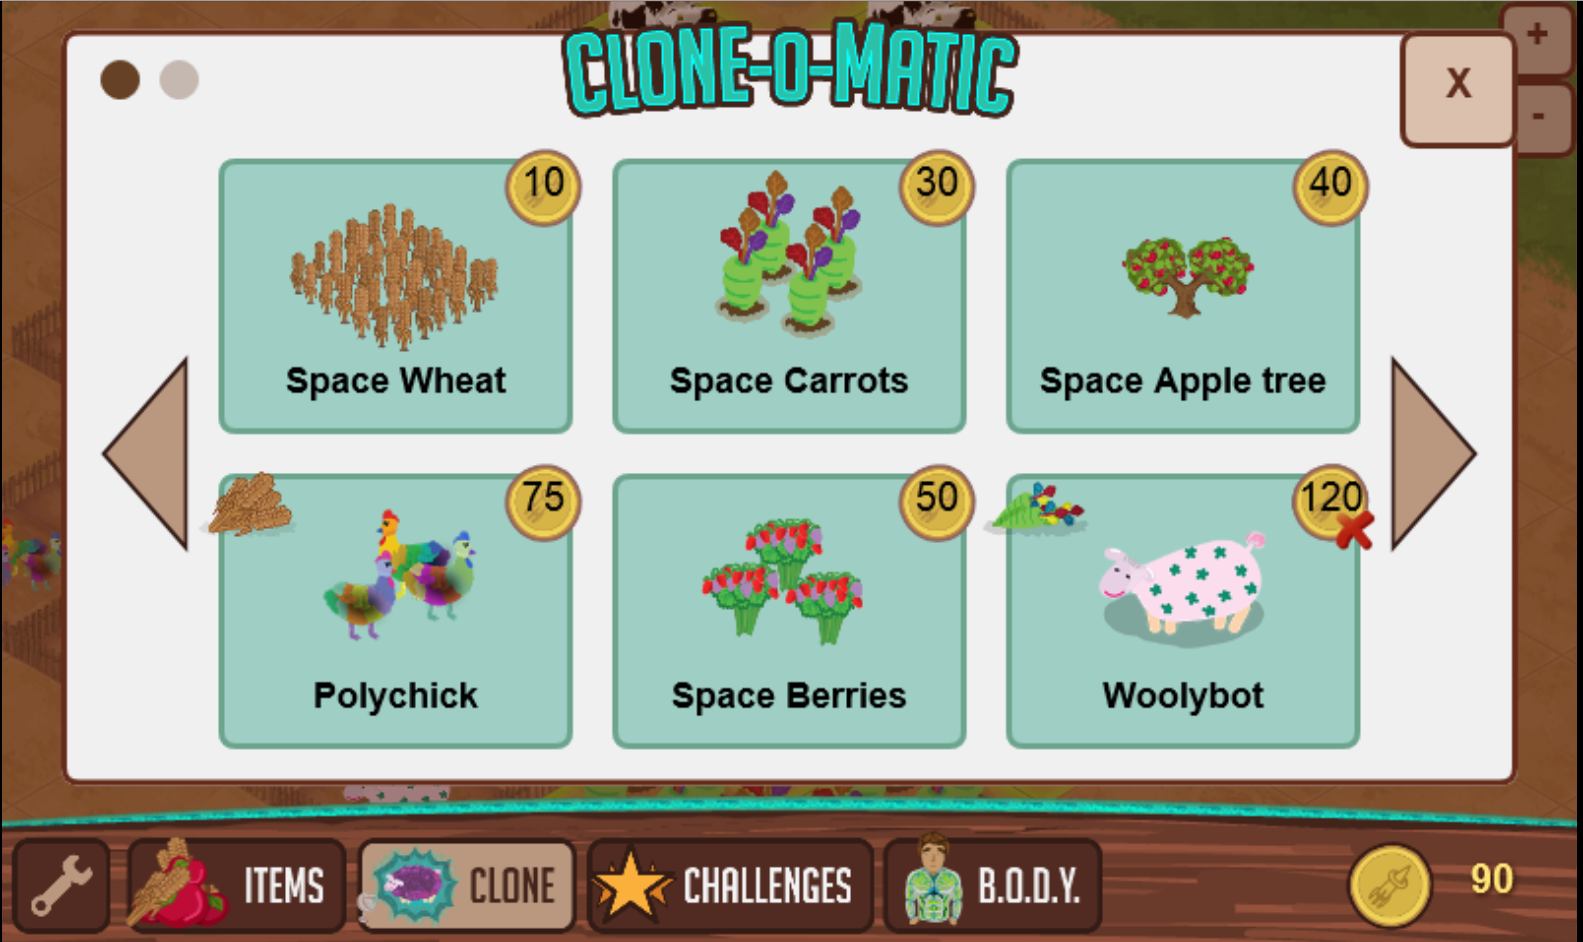
\includegraphics[width=0.80\textwidth]{images/cloning.png}
	\caption{Cloning crops / livestock}
	\label{fig:cloning}
\end{figure}

\paragraph{Available crops (cost, time to grow [minutes], revenue of single harvest, number of harvests)}
\begin{itemize}
\item Space Wheat (10, 10, 15 + 1 space wheat, 1)
\item Space Carrots (30, 45, 50 + 1 carrot, 1)
\item Spaceapple tree (40, 20, 25 + 1 space apple, 3)
\item Space Berries (50, 90, 75 + 1 space berry, 1)
\item Diamond Spirulina (70, 120, 35 + 1 diamond, 3)
\end{itemize}
\paragraph{Available livestock (cost, time to get ready for exploitation [minutes], revenue of single exploitation)}
\begin{itemize}
\item Polychick (75, 45, 20 + 1 egg)
\item Woolybot (120, 120, 40 + 1 wool)
\item Piggium (200, 240, 75 + 1 bacon)
\item Milkatron (300, 360, 100 + 1 milk)
\end{itemize}

\section{Future Work}
\label{sec:FutureWork}
%3. from prototype to the final game (up scaling)
%- what was left out in the prototype? what's the roadmap to the final game? what are the main
%challenges on that path?
%- (non-technical) recommendations and warnings

This chapter describes the features and goals for a new release of the game which are not implemented in this version due to time restrictions and other reasons. The reason of exclusion from this version is explained at each point.

\subsection{Different play modes}
The current version of the game assumes the user to have a certain goal: making them aware of their lifestyle and stimulate to live more healthy. Also the level of the user is fixed at a person with a low-moderate fitness level.
\\\\
In future versions of the game we aim to focus on more specific types of users with varying goals. The exercises and challenges are then adjusted to this goal. The option to choose a more personalized goal should create a certain amount of trust that the game helps the user to reach that goal. This could motivate the user even more to execute all the exercises. 

\subsection{Exercises}
In the current version, active players are able to plant all crops and livestock within several days, not long after they will have finished all challenges at least once. To work towards a final game, more challenges, crops, livestock and levels have to be offered to keep the game engaging. All of these features depend on \textit{exercises}, so also plenty more exercises should be selected and implemented to keep the game engaging and fun. 
\\\\
Moreover, exercising is what this game is about and varying exercises is important to train different types of muscles within a body part. Additional exercises have to be selected in further cooperation with a physiotherapist to make a well considered offer of them within the game.

\subsection{Events}
In the original game design document we planned to introduce events to the game. A quote from the original design document:
\textit{``Events will occur randomly in the game and are used to create extra challenges for the player. An example of an event is a raid of Space Cowboy to the farm or a disease that comes to your planet. More severe events will happen once the player has reached a higher level. The chances of getting events will decrease when the player is active.''}
This however was never a high priority and due to time reasons this feature is never implemented. In future versions however it could enrich the gameplay and adjust the difficulty to the success of the player better to keep the player in the flow, see figure~\ref{fig:gamedifficulty}. According to research the game should therefore not be too difficult nor too easy. Inserting events at the right time can make the game harder respectively easier when the game is too easy respectively too hard for the player. 

\begin{figure}[h]
	\centering
		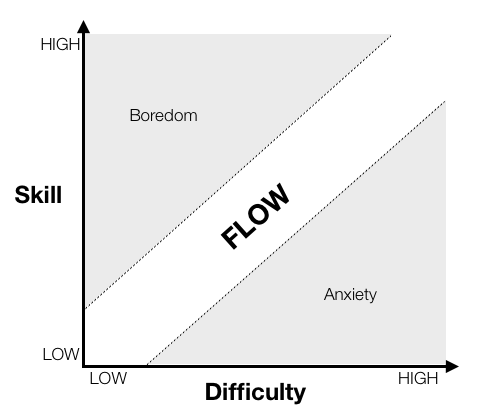
\includegraphics[width=0.60\textwidth]{images/DynamicGameDifficulty.png}
	\caption{Flow, boredom, and anxiety as they relate to task difficulty and user skill level. (2015, January 14). Retreived from: http://www.gamasutra.com/view/feature/166972/, by Csikszentmihalyi, 1990}
	\label{fig:gamedifficulty}
\end{figure}

\subsection{Market}
In the original game design we planned to include a market. A quote from the original design document describes the initial purpose:
\textit{``From the farm you are able to see your inventory. Here you will have an overview of all the items you currently possess. These items can be sold on the market, giving you the revenue they are worth.''}
This feature did not have a high priority at first, as you use the items to start challenges and receive money right away when you harvest. Including the market in the game however provides guidance to the user since it needs certain crops and challenges to be done. 

\subsection{Make body interactive}
\textit{Information is motivation}, from this point of view it would be good to provide more information about the body parts and the use of exercises. One of the future features should therefore provide information about the muscle when it is clicked on in the BODY menu. Next to more information also the challenges and crops that use these muscles have to be shown to make it easy for the user to find the exercises meant for a specific body part. 

\subsection{Statistics Graph}
The BODY menu gives the option to see the statistics to see the completed exercises in the past. To make these statistics more easy to analyse they have to be visually shown with a graph, showing a summary of the gained experience points per body part for a time interval selected by the user. By clicking on a certain point in the graph the finished exercises at that point should be shown.

\subsection{Disclaimer}
The game needs the user to execute all kinds of exercises without prior physical and medical tests. The responsibility of performing the exercises and possible injuries should therefore lay with the user. To warn the users about possible consequences, although they are limited to the minimum, and indicate that the game is on their own responsibility, this should be mentioned in the disclaimer. 

\subsection{Some more fun}
To indicate that the game could really improve the fitness of the user an example would be nice to have. What example is better than the already introduced Phil, an old man in good shape. We planned to look for ``an old photo'' of our example from the time before he was exercising and while he was exercising. With his extensive experience he can tell about his experience and what he had to do to reach and maintain his current shape. 

\subsection{Personal calibration}
People like a personal approach, not feeling just one among many. A personal approach could motivate the user and could also lead to faster results. The intended personalisation consists of a calibration to adjust the settings considering for example the age, height, arm length, weight, current fitness, etc. This information is first of all usable to improve the precision of the measurement of the sensors. Besides that, also the amount of repetitions of exercises, the types of exercises and feedback could be adjusted.

\subsection{Materials}
Giving the users more freedom to decide what they want could increase fun and engagement. Once users earned plenty of money they should be able to invest it to speed up processes and improve faster. This is why we want to introduce materials. Materials can be bought and help speeding up or unlocking certain processes. For example, buying a plowvercraft speeds up the processes on the farm and therefore a crop could be harvested earlier. 

\end{document}
